\section{Resources}

Two core features of rural landscapes are vegetation and water networks. Accurately replicating these features is therefore critical to the resulting realism of the modelled virtual world.\\
The combination and annual variance of temperature, illumination and precipitation have a direct effect on vegetation and water networks. Therefore, to procedurally determine the vegetation and water networks, available resources must first be resolved. This section will focus on the approach taken to determine available resources throughout the terrain. Due to scope, not all resources could be modelled and this work focuses on: \textit{Illumination}, \textit{temperature}, \textit{precipitation}, \textit{soil humidity} and \textit{slope}. 

\subsection{Illumination}

Illumination and annual variation thereof greatly effects the type and density of vegetation that can grow. Whereas some plants prefer habitats with limited sunlight exposure (lilies, etc.), some strive in fully exposed environments (sunflowers, etc.). \\
To determine whether or not a point on the virtual terrain is illuminated at any given time of the year, the system must be able to track the suns trajectory through time. How this is done and how the terrain illumination is calculated accordingly is discussed below.

\subsubsection{Calculating the suns trajectory}

The earth rotates around the sun with an axial tilt, also known as obliquity, of approximately 23.5 degrees (see figure \ref{fig:earth_orbit}). Because of this obliquity, given a position \textit{X} at latitude \textit{L}, the amount of illumination received at \textit{X} in a a 24-hour period will vary during the course of a year (see figure \ref{fig:daylight_variation}). For the northern hemisphere, the day length will be at it's maximum during the June equinox and at it's minimum during the December equinox. At these moments in time, the earth will be tilted at it's maximum towards and away from the sun respectively.\\

\begin{figure}
\center
	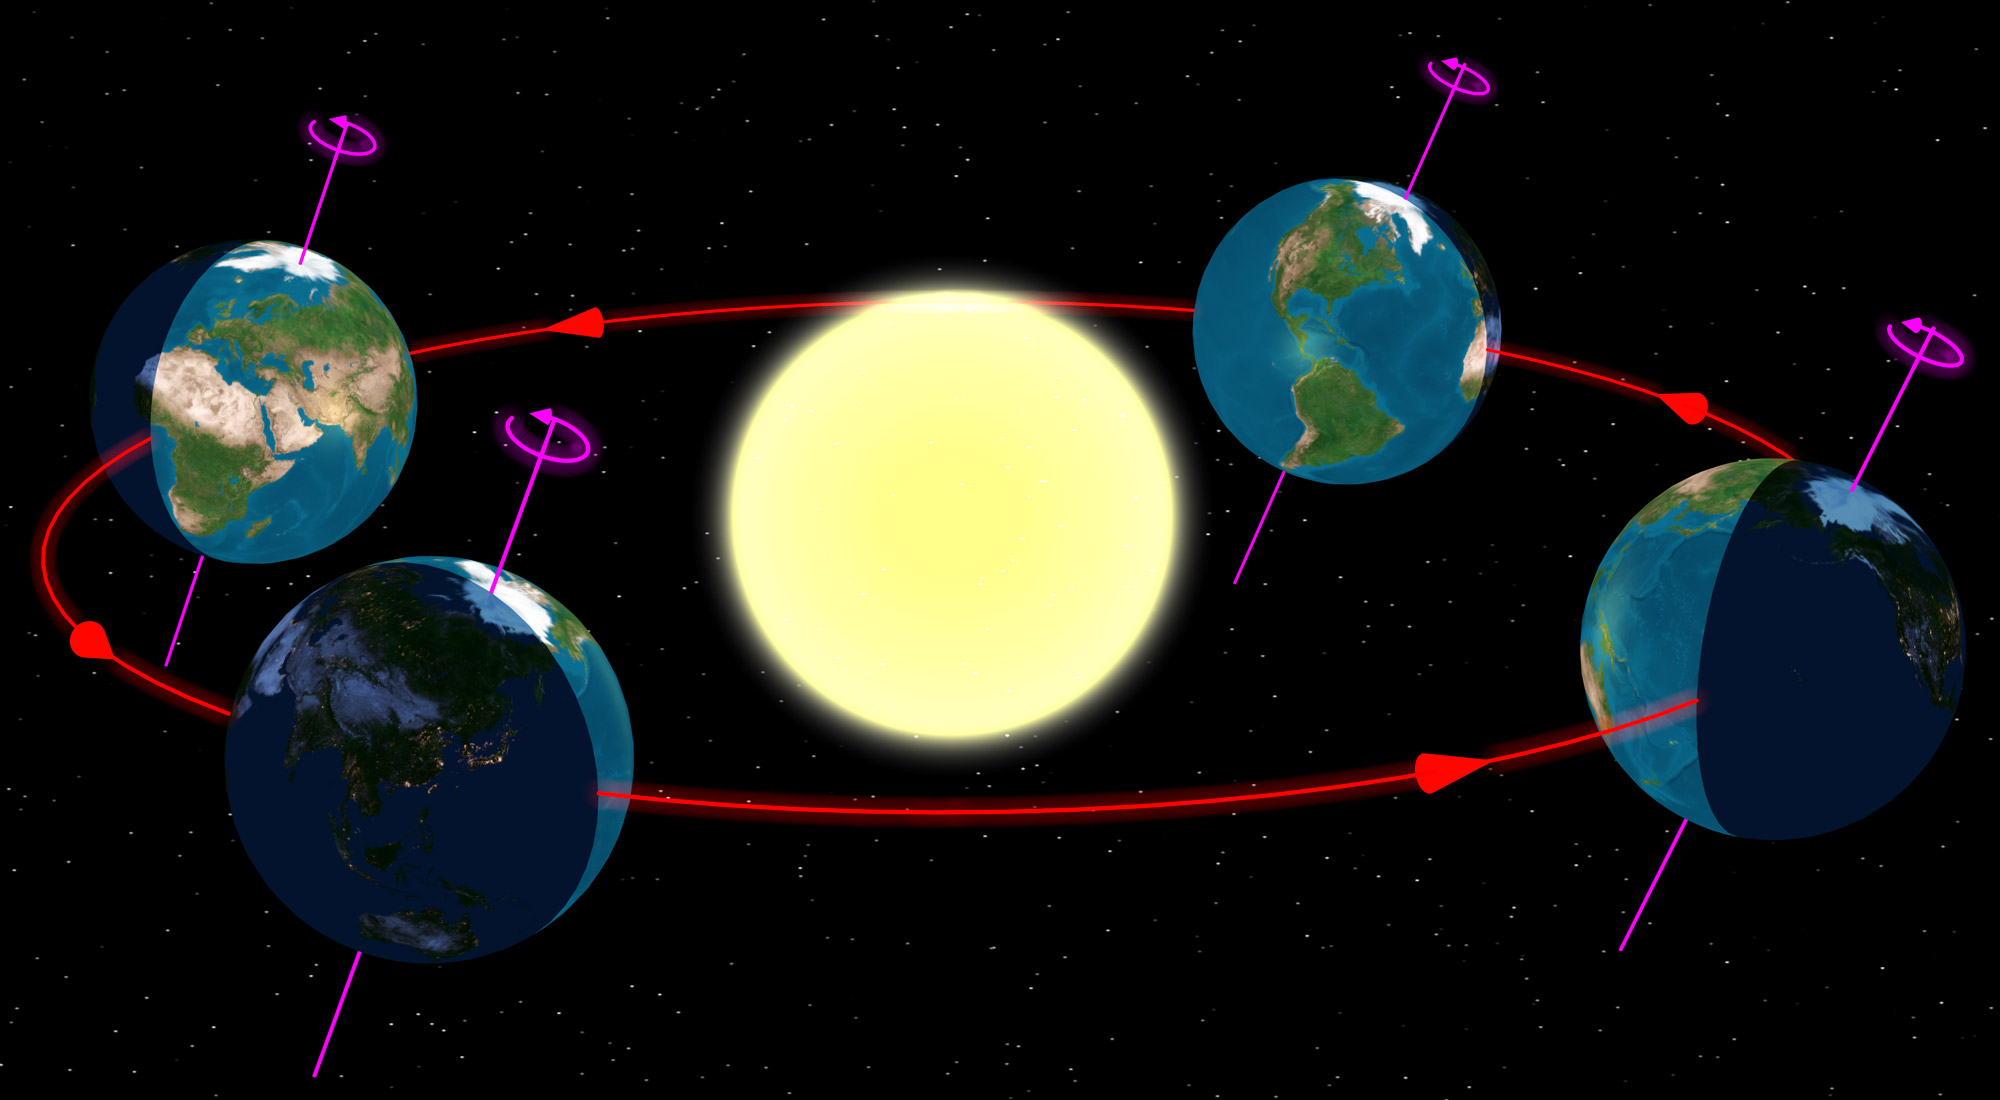
\includegraphics[width=\textwidth]{earth_orbit.jpg}
	\caption{ Earth orbiting the sun \protect\footnotemark}
	\label{fig:earth_orbit}
\end{figure}
\footnotetext{\url{http://en.wikipedia.org/wiki/Summer_solstice}}

\begin{figure}
\center
	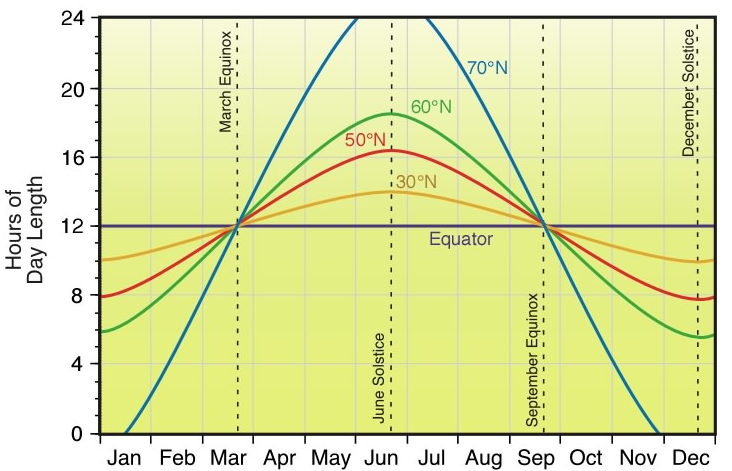
\includegraphics[width=\textwidth]{daylight_variation.png}
	\caption{ Variation in day length for different latitudes \protect\footnotemark}
	\label{fig:daylight_variation}
\end{figure}
\footnotetext{\url{http://www.physicalgeography.net/fundamentals/6i.html}}

In order for the terrain to remain static, when calculating the sun's trajectory the frame of reference is changed to be the earth, around which orbits the sun. To calculate the sun's position at any given time, there are four vital pieces of information that need to be specified by the user: \textit{Latitude}, \textit{Orientation}, \textit{Time of day} and \textit{Month of year}. \\

Specifying the \textit{latitude}, \textit{time of day} and \textit{month of year} is done using sliders which overlay the rendering window (figure \ref{fig:lat_and_time_control}). By keeping the render window visible during this edit, modifications are clear to the user. When any of these values are changed, the position of the sun is automatically recalculated in real-time. \\

\begin{figure}
\center
	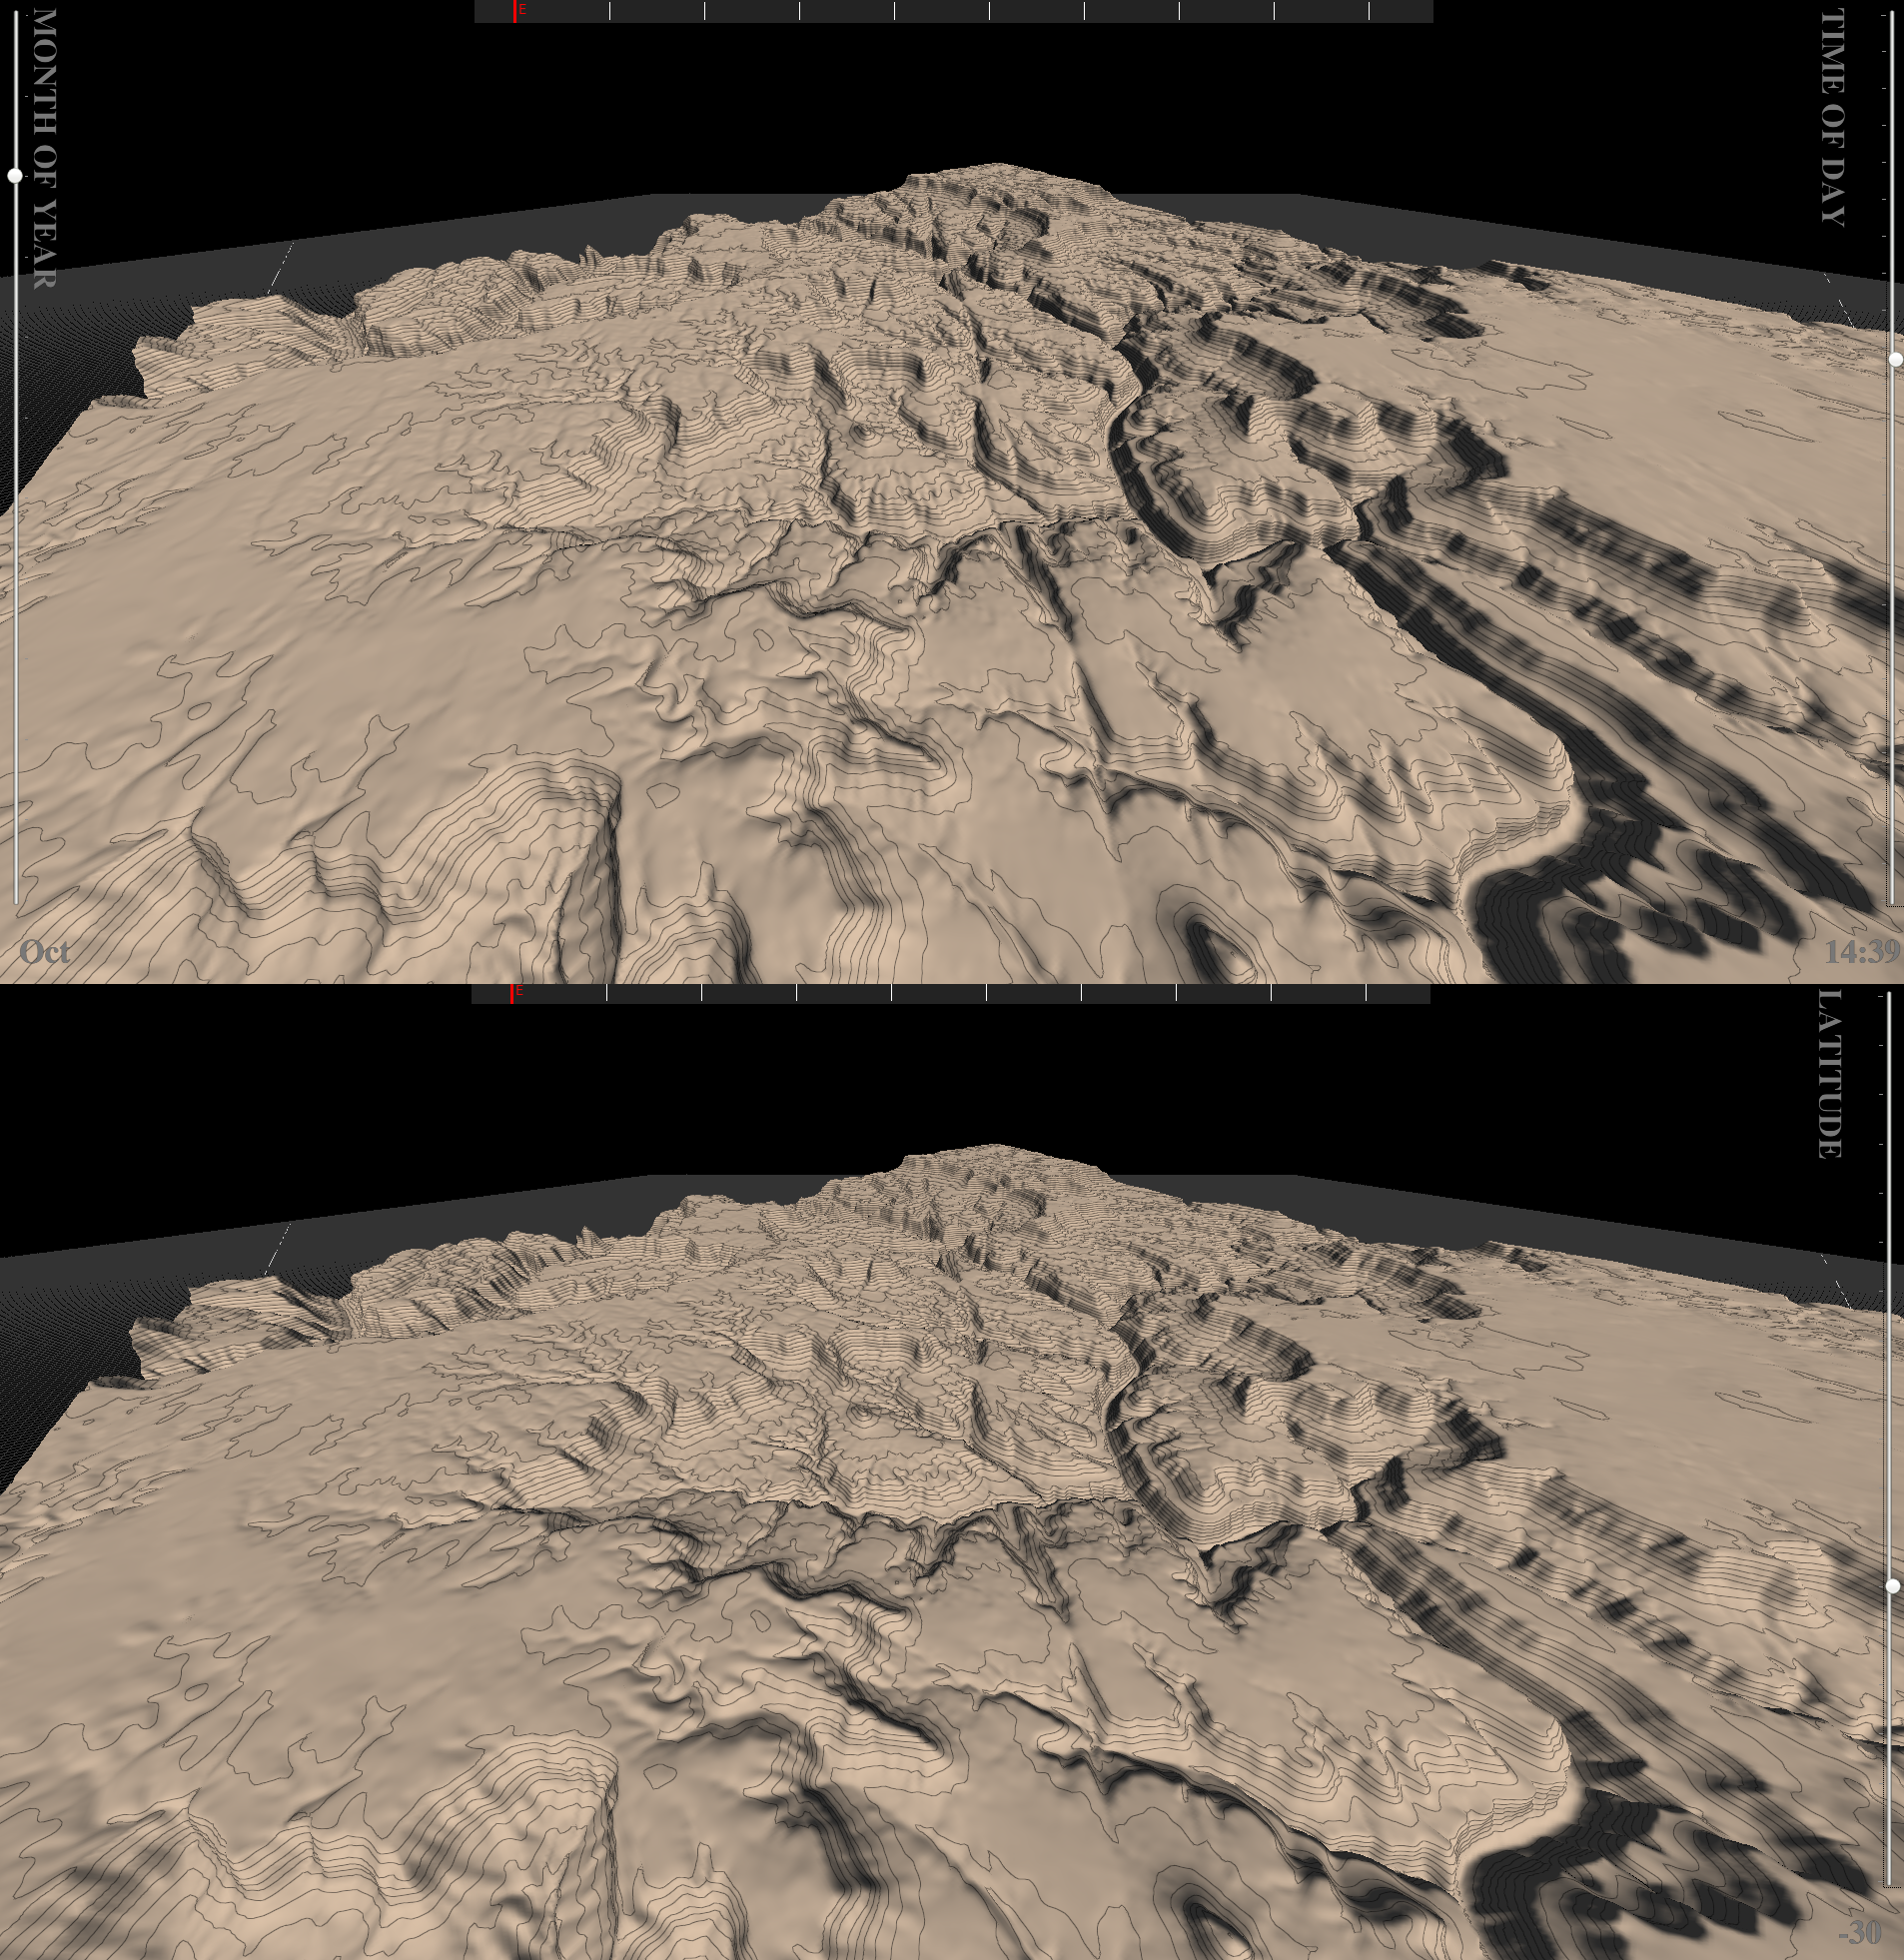
\includegraphics[width=\textwidth]{controlling_time_and_latitude.png}
	\caption{ Time (top) and latitude (bottom) controllers }
	\label{fig:lat_and_time_control}
\end{figure}

Orientation is displayed to the user at all times with the use of an overlay compass (figure \ref{fig:orientation_control}) inspired by first-person video games. When in "orientation edit mode" the compass changes to green to inform the user edit mode is active, at which point the orientation can be modified by using the right/left keyboard keys. Again, all modifications update the sun position in real-time.\\

\begin{figure}
\center
	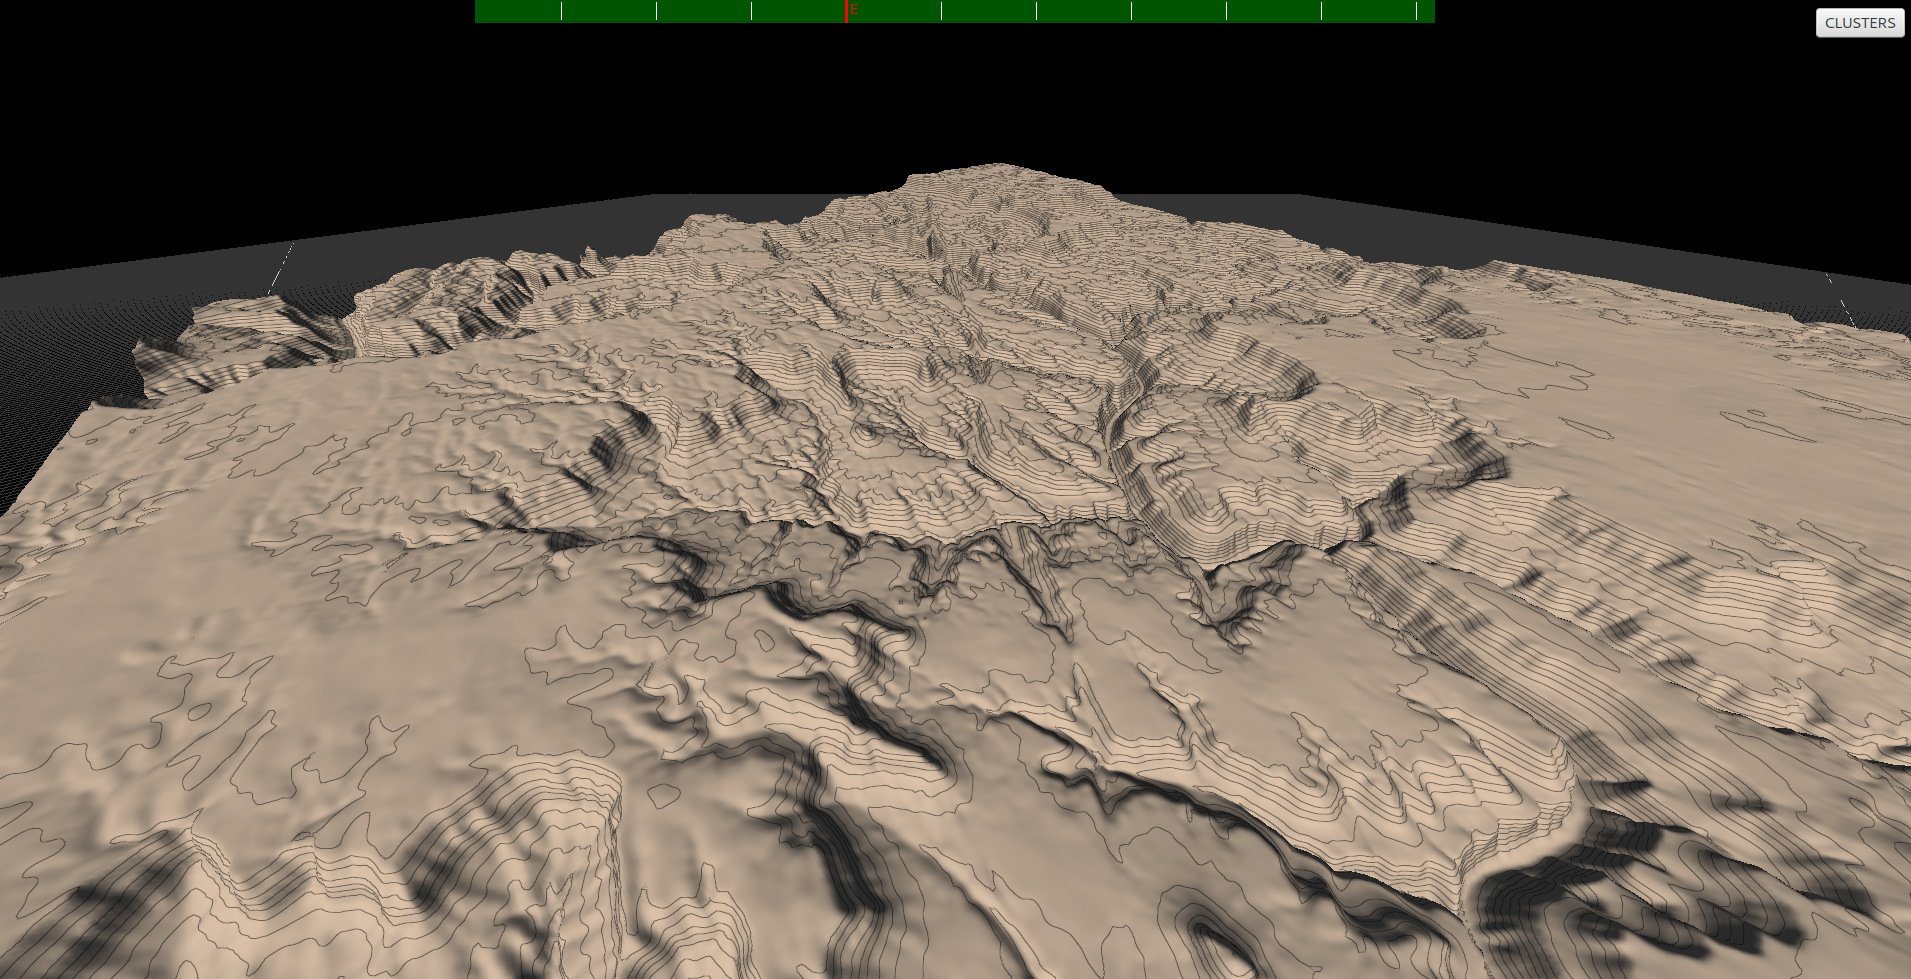
\includegraphics[width=\textwidth]{orientation_controller.png}
	\caption{ Orientation controllers}
	\label{fig:orientation_control}
\end{figure}

Given all this information, the first step is to calculate the rotation axis \textit{V$_{RE}$} of the sun at the equinox. This is done using equation \ref{eq:equinox_rotation_axis}. Taking \textit{V$_{RE}$} as the rotation axis for the sun is a simplification. However, the distance between earth's center axis and \textit{V$_{RE}$} is negligible in comparison to the distance between the earth and the sun and is therefore deemed an acceptable simplification.\\

\begin{equation} \label{eq:equinox_rotation_axis}
	V_{RE} = R(V_{N}, \textit{-L}, V_{E})
\end{equation}
where:
\begin{itemize}
\item \textit{V$_{RE}$} is the rotation axis of the sun at the equinox.\\
\item \textit{V$_{N}$} is the north-facing vector passing through the terrain center.\\
\item \textit{V$_{E}$} is the east-facing vector passing through the terrain center.\\
\item \textit{L} is the latitude of the terrain.\\
\item \textit{R(V$_{a}$,\textit{a},V$_{b}$}) is the resulting vector after rotating V$_{a}$ by \textit{a} degrees around V$_{b}$\\
\end{itemize}

\textit{V$_{RE}$} is the rotation axis for the sun at the March and December equinox. During the equinox, axis tilt has no effect on daytime duration as the tilt is not directed away or towards the sun. At this point, only latitude is the determinant factor of daytime duration. In order to calculate the rotation axis V$_{R}$(m) of the sun at month \textit{m}, axis tilt must be taken into consideration by further rotating $V_{RE}$ using equation \ref{eq:all_month_rotation_axis}.

\begin{equation} \label{eq:all_month_rotation_axis}
	V_{R}(m) = R(V_{RE}, a_{m}, V_{E})
\end{equation}
where:
\begin{itemize}
\item \textit{V$_{R}(m)$} is the rotation axis of the sun at month \textit{m}.\\
\item \textit{V$_{RE}$} is the rotation axis of the sun at the equinoxes (equation \ref{eq:equinox_rotation_axis}).\\
\item \textit{V$_{E}$} is the east-facing vector passing through the terrain center.\\
\item \textit{a$_{m}$} is the rotation angle calculated using equation \ref{eq:rotation_angle_calculation} .\\
\item \textit{R(V$_{a}$,\textit{a},V$_{b}$}) is the resulting vector after rotating V$_{a}$ by \textit{a} degrees around V$_{b}$\\
\end{itemize}

The time of day, \textit{t} is then used to determine the amount the sun is rotated around the rotation axis \textit{V$_{R}$(m)}. With a full rotation being performed every 24 hours.

\begin{equation} \label{eq:rotation_angle_calculation}
	a_{m} = -tilt_{max} + |6-m| \times tilt_{monthly} $$\\
$$
tilt_{monthly} = tilt_{max}/3
\end{equation}

where:
\begin{itemize}
\item \textit{$a_{m}$} is the rotation angle at month \textit{m}
\item \textit{$tilt_{max}$} is the maximum axis tilt of the earth (~23.5 degrees)
\end{itemize}

\subsubsection{Calculating Illumination}

A point on the terrain is illuminated if there is a direct path from it to the sun with no intersections with other points on the terrain. To test for this on the terrain ray casting is performed from each vertex position towards the sun to check whether or not it intersects with other points on the terrain.\\
A spherical hierarchical acceleration structure is used to accelerate the ray casting process. This hierarchical acceleration structure acts as a tree structure to iteratively search for smaller intersection areas. Using this acceleration structure, illumination can be calculated for 4 million vertices (2048 by 2048 terrain) in just over 2 seconds (figure \ref{fig:illumination_calculation_time}). As shown in figure \ref{fig:illumination_calculation_time}, There is a linear relationship between vertex count and calculation time. (i.e vertex count).

\begin{figure}
\center
	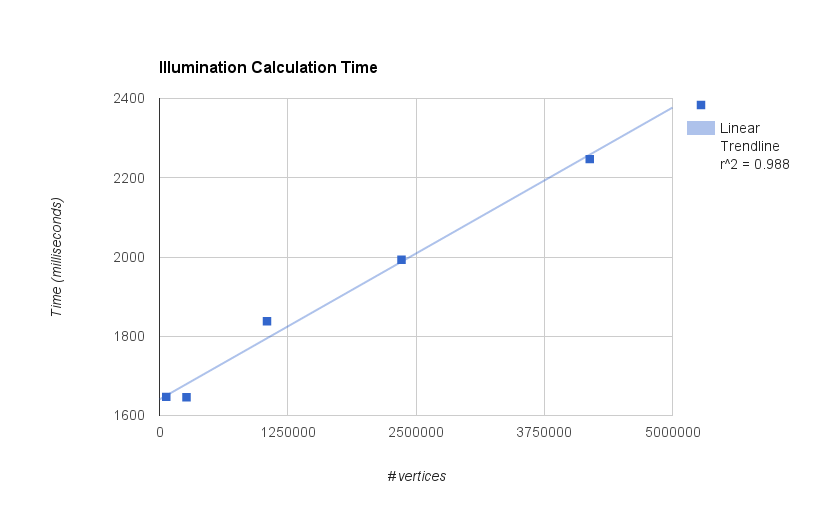
\includegraphics[width=\textwidth]{illumination_calculation_time.png}
	\caption{ Illumination calculation time based on vertex count. Analysis performed for terrains with dimensions: 256 by 256, 512 by 512, 1024 by 1024 and 2048 by 2048. }
	\label{fig:illumination_calculation_time}
\end{figure}

\subsubsection{Illumination overlay} \label{subsub:illumination}

To visually present terrain illumination to the user an \textit{illumination overlay} can be selected which renders an overlay on-top of the terrain (see figure \ref{fig:overlay_illumination})

\begin{figure}
\center
	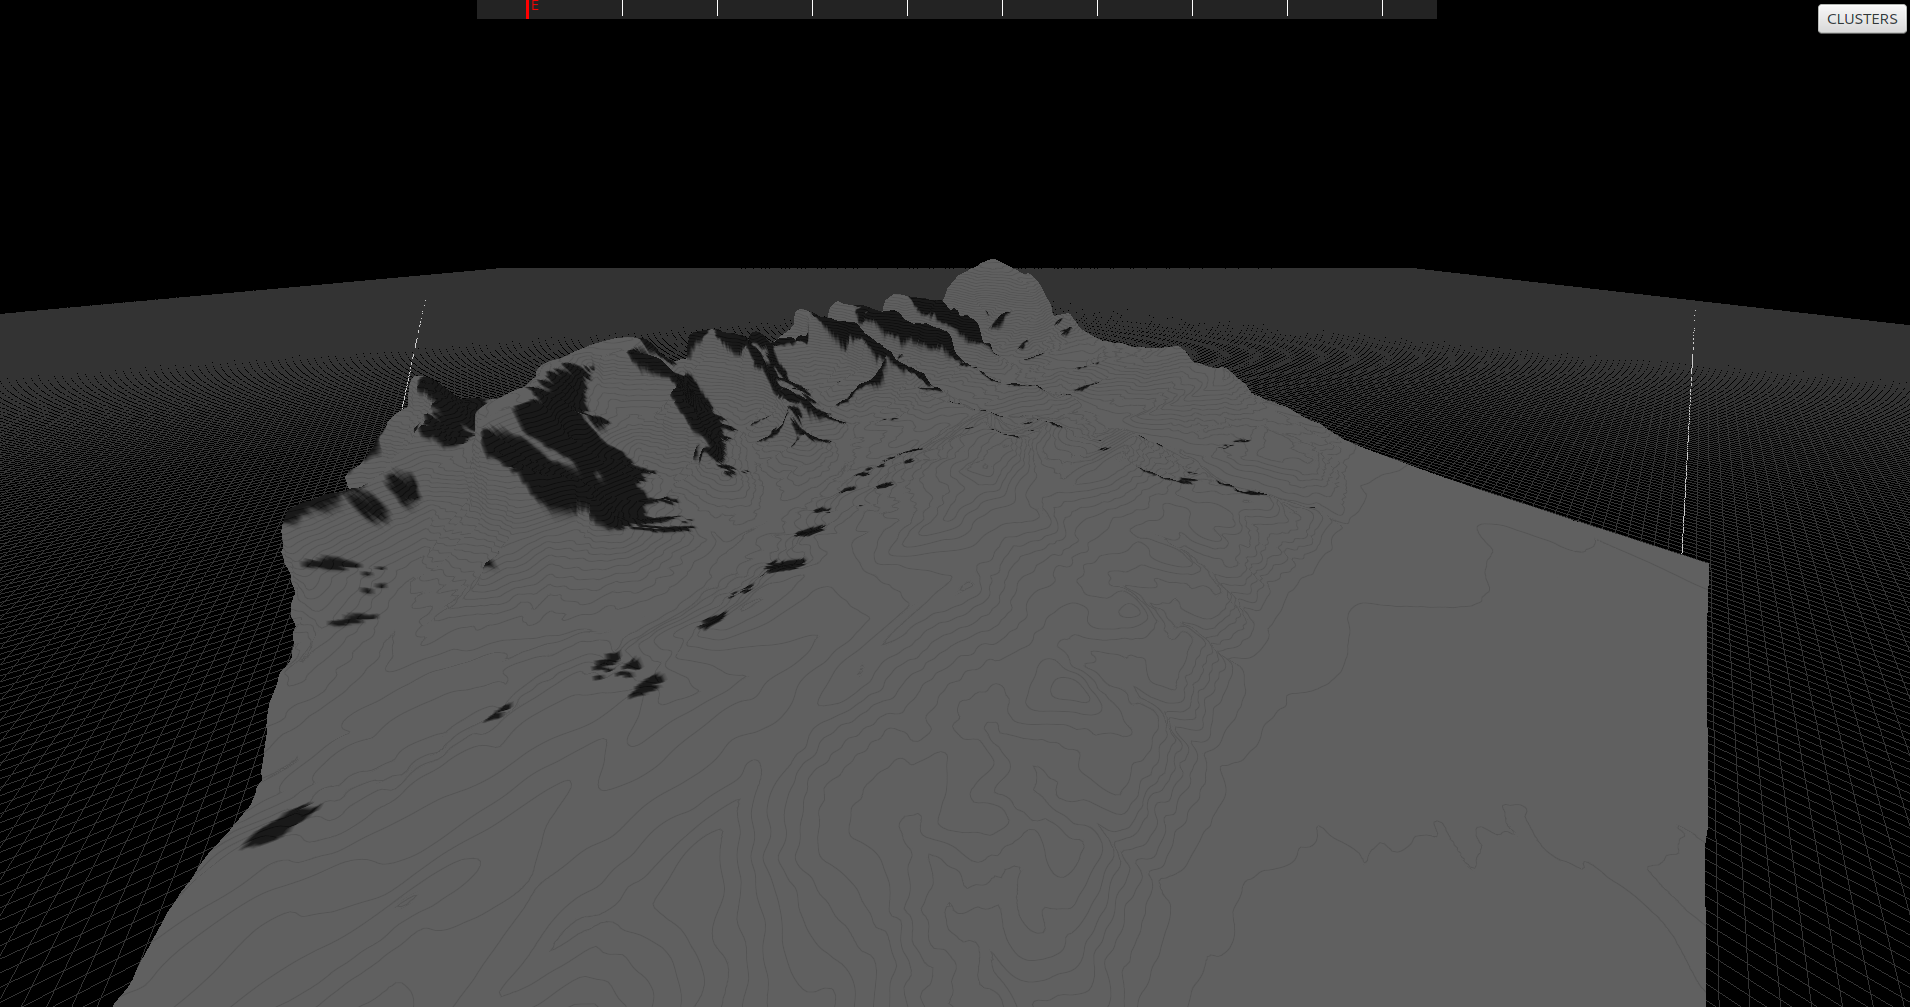
\includegraphics[width=\textwidth]{illumination_overlay.png}
	\caption{ Illumination overlay. Illuminated areas are coloured white. Shaded areas are coloured black. }
	\label{fig:overlay_illumination}
\end{figure}

\subsubsection{Daily Illumination}

An important factor for plant growth is the hours of illumination received throughout the day. The illumination calculation is used (\ref{subsub:illumination}) to determine this by going through each hour of the day consecutively and determining whether or not a vertex \textit{V} is illuminated. 

\subsubsection{Daily Illumination overlay}

Similarly to the illumination, a visual presentation of the daily illumination can be enabled as observed in figure \ref{fig:overlay_daily_illumination}.

\begin{figure}
\center
	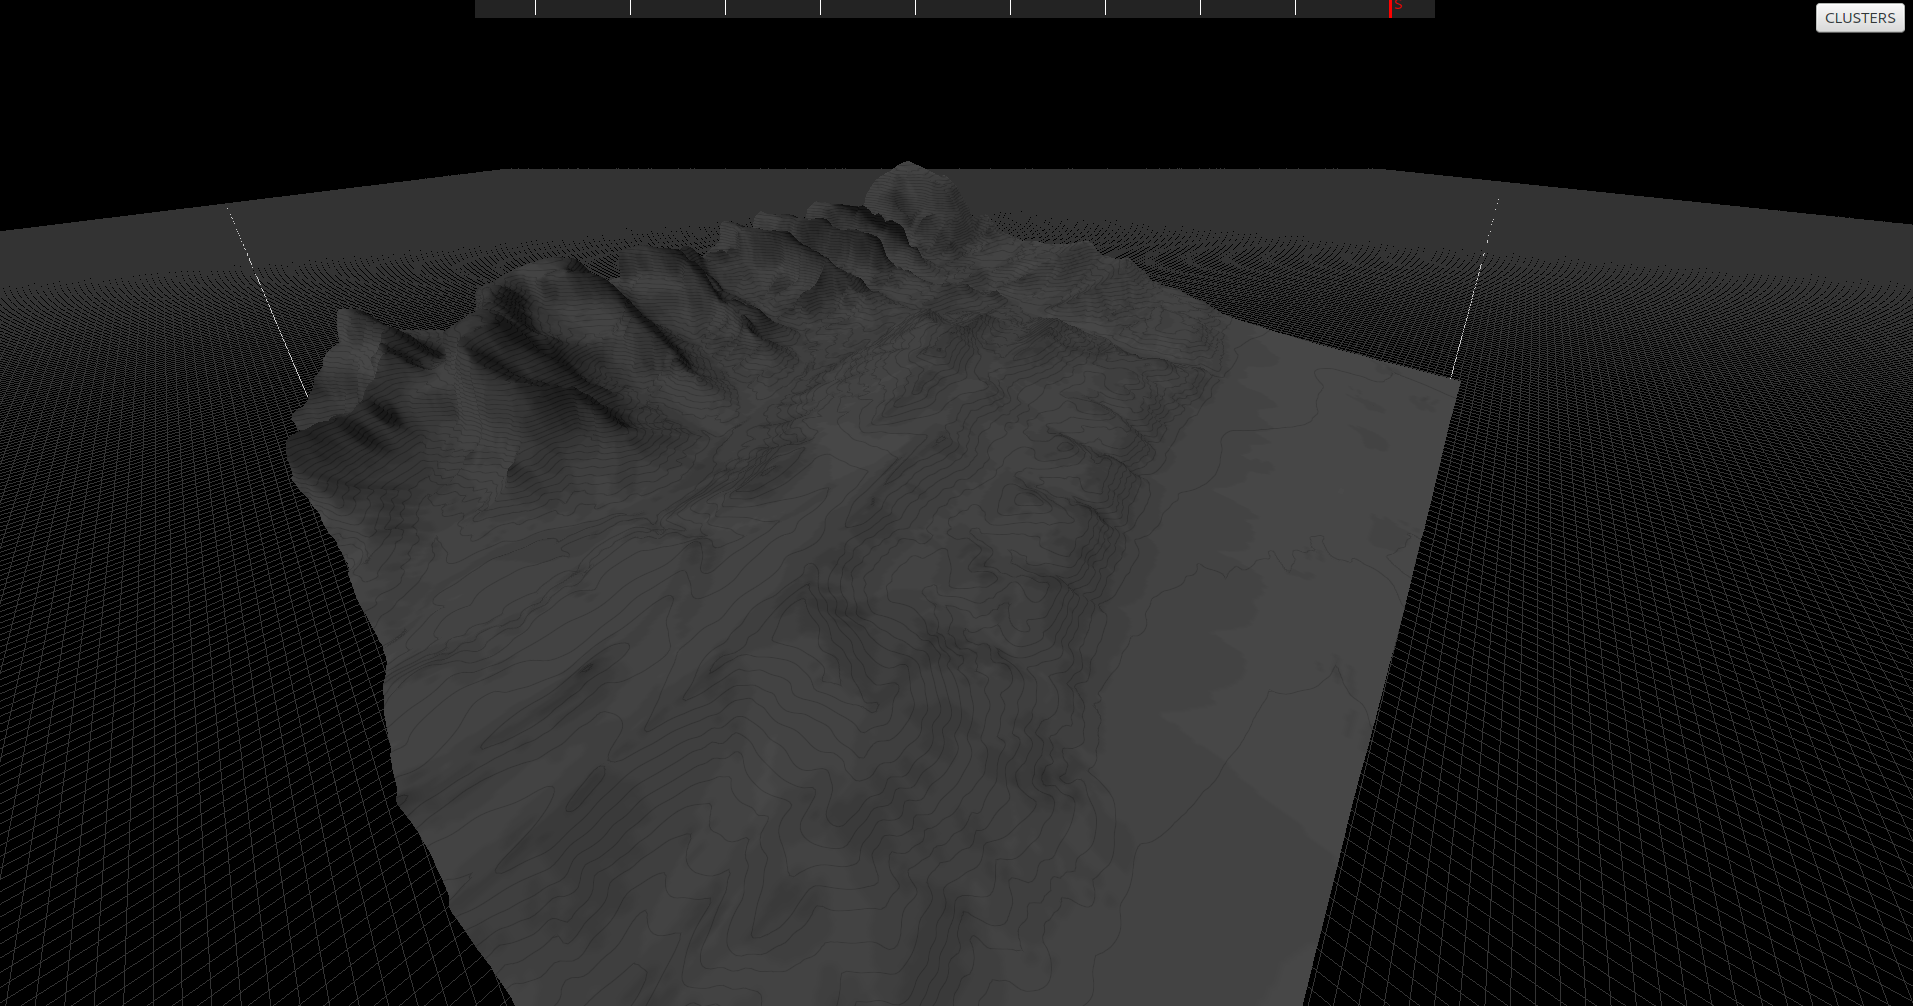
\includegraphics[width=\textwidth]{daily_illumination_overlay.png}
	\caption{ Daily illumination overlay. The brighter the area, the more illumination it receives throughout the day. }
	\label{fig:overlay_daily_illumination}
\end{figure}

\subsection{Temperature}

Whereas tropical climates often have relatively constant temperatures throughout the year, others, such as the continental climate, are characterized by a strong variation between minimum and maximum annual temperatures. Only plants which are able to survive at both extremes can grow which is why temperature and variation thereof has a big impact on vegetation. For modelling purposes, it is acceptable to assume that the minimum temperature, \textit{T$_{min}$}, occurs in the middle of winter and the maximum temperature, \textit{T$_{max}$}, occurs in the middle of summer. Interpolation can be performed to determine the temperature at any time between these two dates.\\

Properties which affect temperature and are necessary to model temperature in the system are: \textit{Altitude}, \textit{Temp$_{december}$}, \textit{Temp$_{june}$} and \textit{Lapse rate}. The \textit{altitude} of each point on the terrain is calculated automatically based on the loaded height-map. Temp$_{december}$ and Temp$_{june}$ represent both extremes of the temperature spectrum at zero meters of altitude and need to be configured by the user. The \textit{lapse rate} defines the decrease in temperature with altitude. Although this changes depending on atmospheric conditions, the default is configured to be 6.4 degrees Celsius for each km of altitude gained. This is accepted as the average atmospheric lapse rate under normal atmospheric conditions \protect\footnotemark.\\
\footnotetext{\url{http://en.wikipedia.org/wiki/Lapse_rate}}

Given this information, the temperature is calculated for any point on the terrain given the month and altitude using equation \ref{eq:temp_calculation}. 

\begin{equation} \label{eq:temp_calculation}
	T(a,m) = T_{december} + ( \frac{6 - |6-m|}{6} \times (T_{june} - T_{december}))
\end{equation}

where:
\begin{itemize}
\item \textit{T(a,m)} is the temperature at altitude \textit{a} and month \textit{m}.
\item \textit{$T_{december}$} is the temperature at zero meters in December.
\item \textit{$T_{june}$} is the temperature at zero meters in June.
\end{itemize}

Calculating the temperature for 4 million vertices (2048 by 2048 terrain ) terrain takes approximately 2 seconds. Figure \ref{fig:temperature_calculation_time} points towards a linear relationship between vertex count and temperature calculation time.

\begin{figure}
\center
	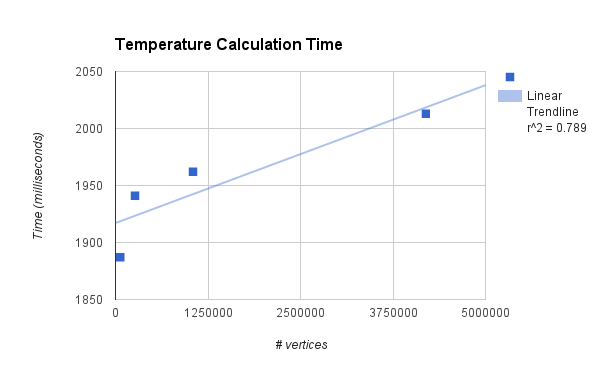
\includegraphics[width=\textwidth]{temperature_calculation_time.png}
	\caption{ Temperature calculation time based on vertex count. Analysis performed for terrains with dimensions: 256 by 256, 512 by 512, 1024 by 1024 and 2048 by 2048. }
	\label{fig:temperature_calculation_time}
\end{figure}

\subsubsection{Temperature overlay}

An overlay can be enabled to get an overview of the temperature at different locations on the terrain (see figure \ref{fig:temp_overlay}).

\begin{figure}
\center
	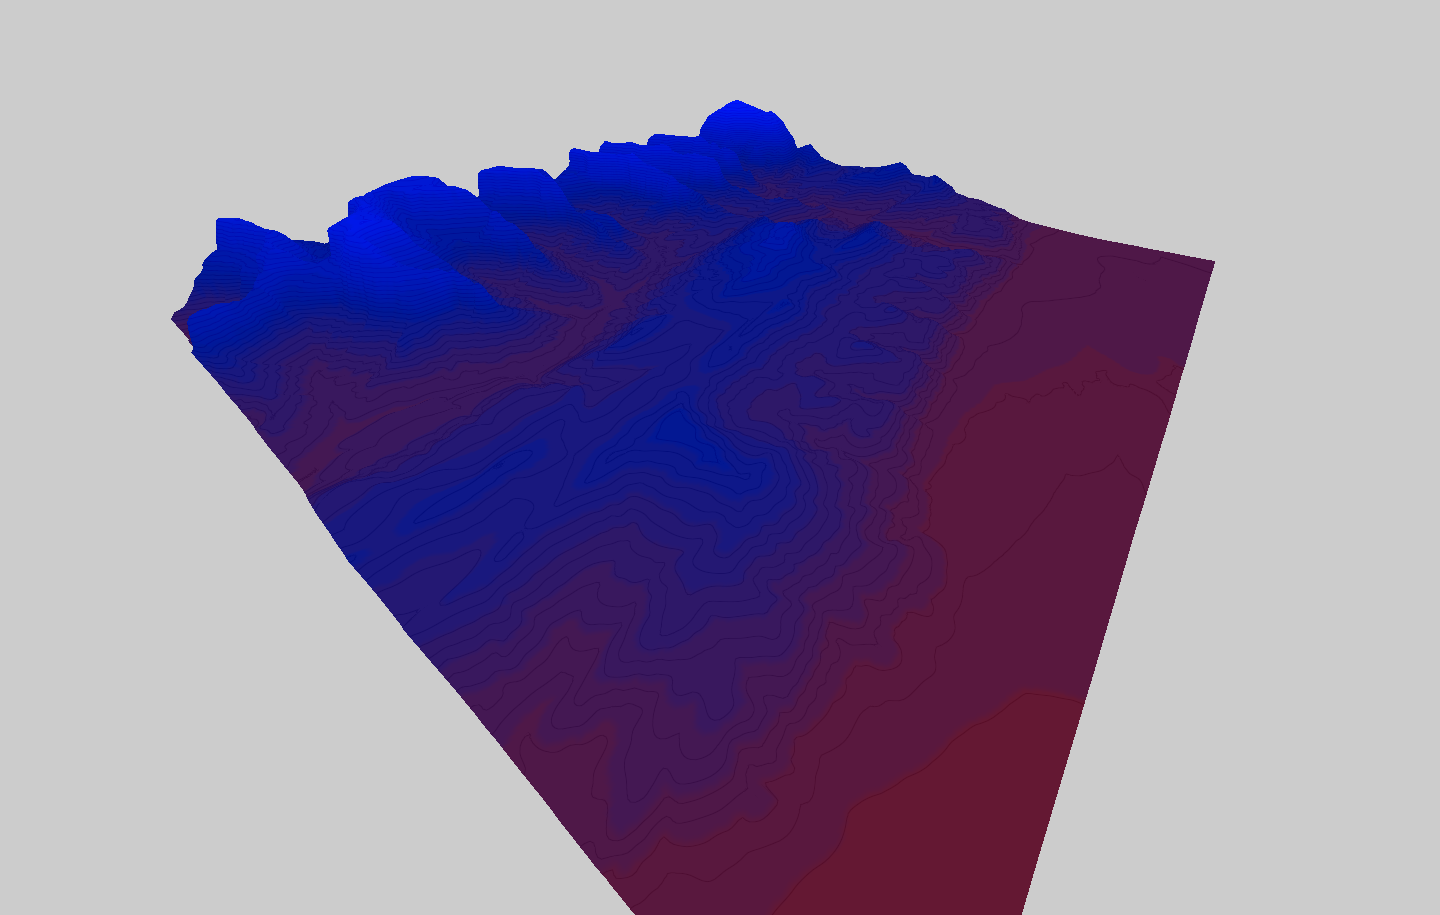
\includegraphics[width=\textwidth]{temp_overlay.png}
	\caption{ Temperature overlay. Colour spectrum ranging from blue (cold) to red (hot). As can be seen, the temperature drops with altitude.}
	\label{fig:temp_overlay}
\end{figure}

\subsection{Precipitation} \label{sec:precipitation}

Precipitation is a core part of climate classification and, consequentially, plant life. Arid climates will have very limited annual precipitation and will be the bottleneck for organic life. Tropical climates, on the other hand, where precipitation is plentiful, has an abundance of vegetation. There are two important properties of precipitation that are modelled: \textit{Quantity} and \textit{Intensity}. The \textit{quantity}, often measured in mm, defines the amount of water which falls. The intensity, often measured in mm/h defines the rate at which it falls.\\

The user must configure \textit{quantity} and \textit{intensity} values for each month of the year. A custom input dialogue was implemented in an attempt to make this as user-friendly as possible (\ref{fig:rainfall_input}).

\begin{figure}
\center
	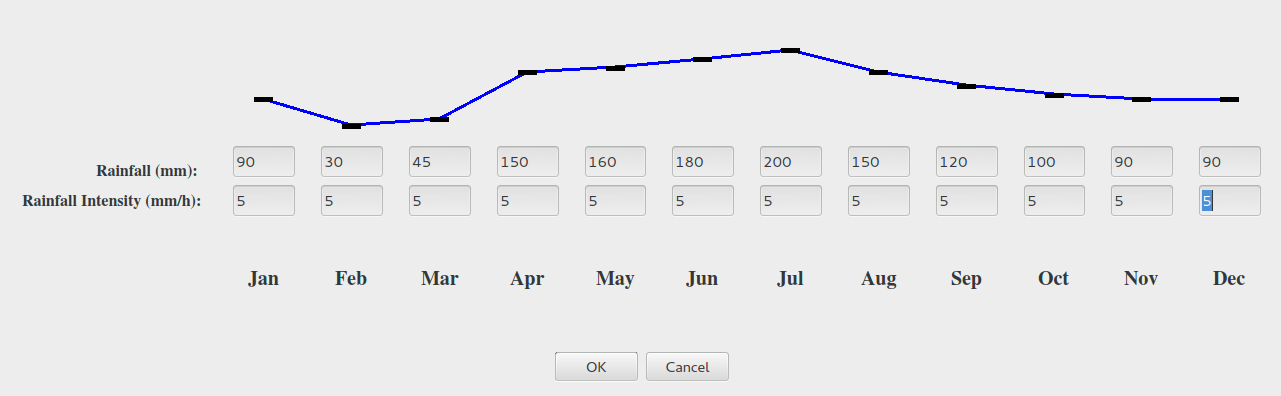
\includegraphics[width=\textwidth]{rainfall_input.png}
	\caption{ Specifying monthly precipitation and precipitation intensity. The user can enter values manually (using the input fields) or interact directly with the graph.}
	\label{fig:rainfall_input}
\end{figure}

\subsection{Soil Humidity}

When rain falls onto the terrain, a certain portion of it is absorbed into the soil to provide the plant's roots with the necessary nutrients. The portion which is absorbed depends on the type of soil. Rocky soils, for example, have limited water retention capabilities and will result in larger water build-up. In this work, the soil humidity is simply a measure, in mm, of the rainfall which is absorbed by the soil. This is determined using the precipitation information outlined above (\ref{sec:precipitation}) along with the \textit{Soil Infiltration Rate}.

\subsubsection{Soil Infiltration Rate}\label{subsubsec:soil_infiltration_rate}

The \textit{soil infiltration rate} is a measure of the quantity of water which can be absorbed in a given time period. If the rainfall intensity exceeds the soil infiltration rate, it will result in water stagnation (flat surface) or water run-off. This rate is correlated with the type of soil and approximate values for some soil types can be found in table \ref{tab:control_types}.

\begin{table}[h]
  \centering
	    \begin{tabular}{|p{5cm}|p{8cm}|}
  	    \hline	
  	    \textbf{Soil-type} & \textbf{Infiltration rate (mm/hour)} \\
		\hline
		\textbf{sand} & $<$ 30 \\
		\hline
		\textbf{sandy loam} & 20-30 \\
		\hline
		\textbf{loam} & 10-20 \\
		\hline
		\textbf{clay loam} & 5-10 \\
		\hline
		\textbf{clay} & 1-5 \\
		\hline
		\end{tabular}
		\caption{Soil infiltration rates for different soil types \protect\footnotemark}
	  \label{tab:control_types}
\end{table}
\footnotetext{\url{http://www.fao.org/docrep/s8684e/s8684e0a.htm}}


Specifying the soil infiltration rate can be done using three distinct tools: \textit{Filling}, \textit{Slope-based} and through a \textit{Painting interface}.\\
Using the \textit{filling} tool, the user can fill the entire terrain with a configured infiltration rate.\\
The \textit{slope-based} tool permits the user to configure a slope above which the soil infiltration rate will be zero. This is an efficient tool for modelling cliff faces or simply areas where water run-off is too severe.\\
The \textit{painting interface} enables user to paint a soil infiltration on the terrain directly using a common brush tool found in basic paint applications. The size of the brush can be configured using the scroll-wheel and the painted soil-infiltration using a dedicated slider controller (\ref{fig:soil_infiltration_controls}).

These tools can be used interchangeably and users are encouraged to do so. Configuring the soil infiltration of the terrain in figure \ref{fig:soil_infiltration_controls}, for example, was performed in approximately three minutes using all three tools as follows:
\begin{enumerate}
\item The filling tool was used to fill the entire terrain with an infiltration rate of 25.\\
\item The slope-based tool was used to set to zero the infiltration rate of all areas with a slope above 30 degrees.\\
\item The painting-tool was used to paint an infiltration rate of zero on the flat area to the right to cater for a water build-up (reservoir, lake, ocean, etc.).\\
\end{enumerate}

\begin{figure}
\center
	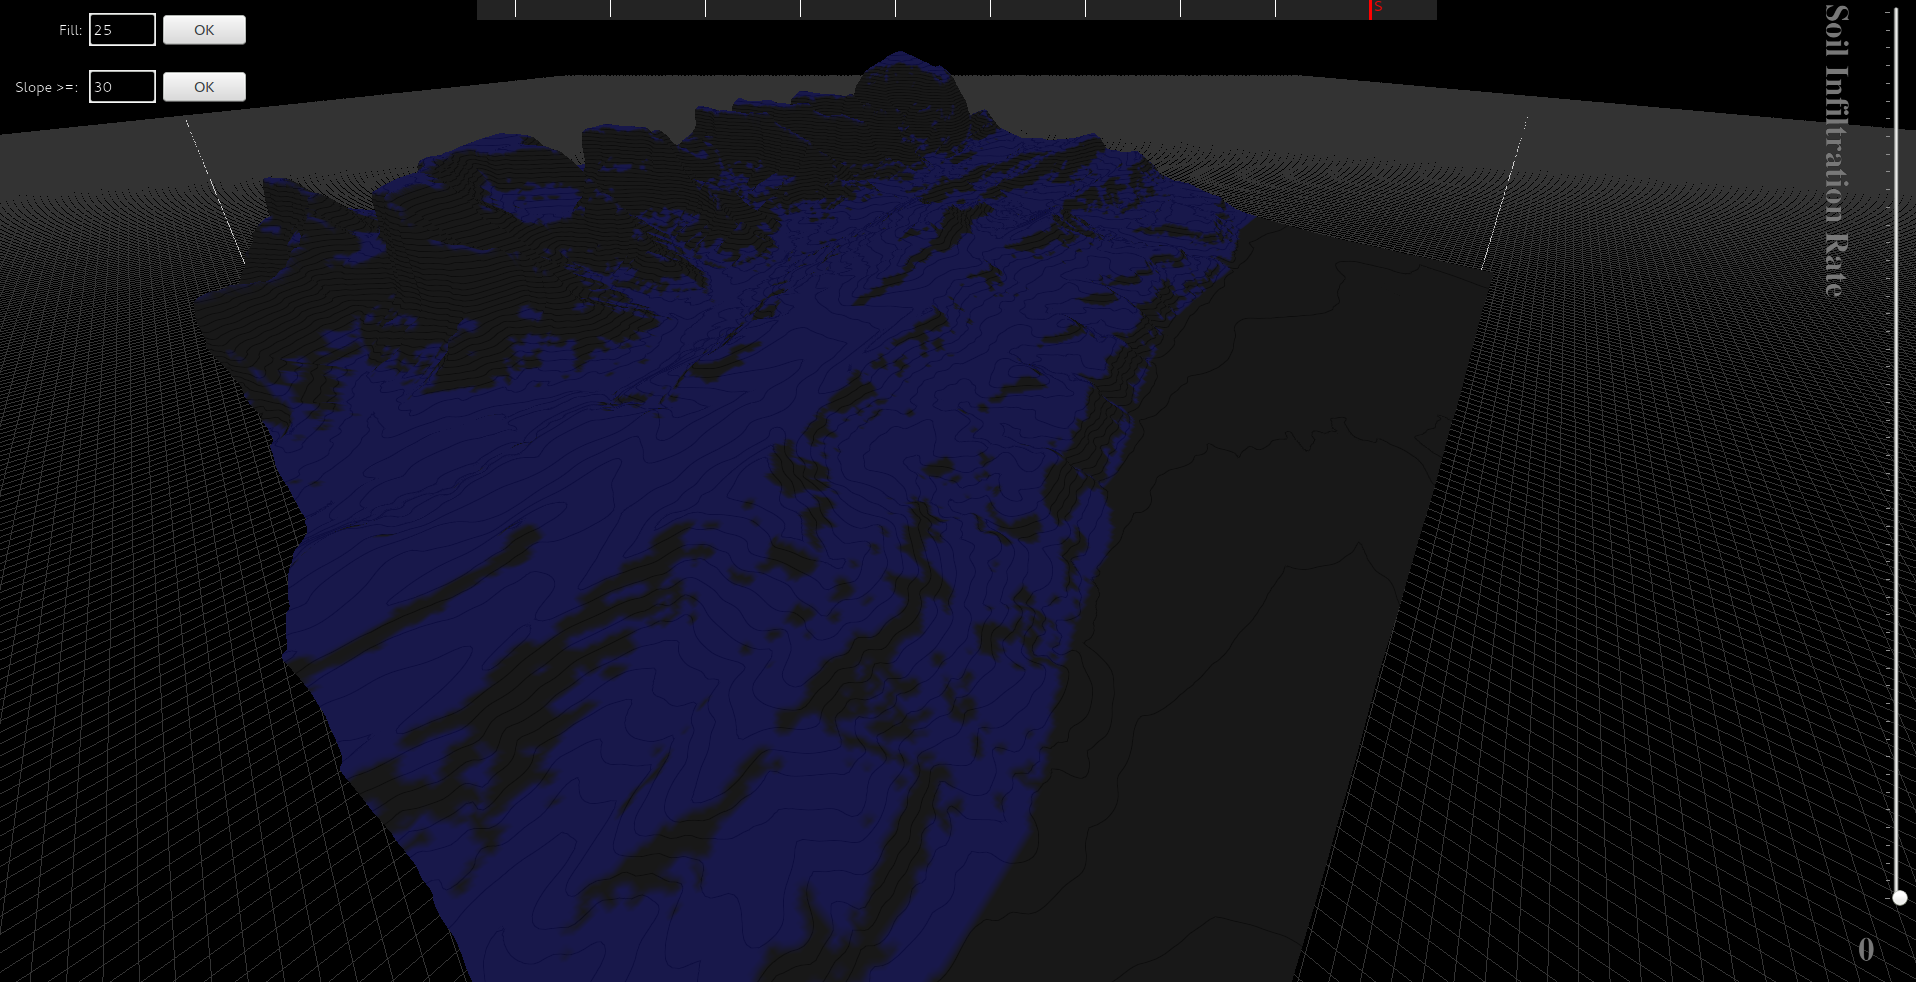
\includegraphics[width=\textwidth]{soil_infiltration_rate_controls.png}
	\caption{ Editing the soil infiltration rate on the terrain. Top left are the controllers for the \textit{filling} and \textit{slope-based} tools. On the right is the slider to configure the soil infiltration rate of the \textit{paint brush}. }
	\label{fig:soil_infiltration_controls}
\end{figure}

\subsubsection{Monthly Soil Humidity Calculation}

Given the \textit{soil infiltration rate}, \textit{monthly precipitation} and \textit{monthly average precipitation intensity} for each vertex on the terrain, it is possible to calculate the quantity of the rainfall which is actually absorbed by the soil for each month. This represents the soil humidity in our system and is calculating using equation \ref{eq:monthly_soil_humidity}. 

\begin{equation} \label{eq:monthly_soil_humidity}
	S_{h}(R_{q},R_{i},S_{ir}) = 
	\frac{S_{ir}}{R_{i}} \times R_{q}
\end{equation}
where:
\begin{itemize}
\item \textit{$S_{h}$} is the soil humidity, in mm.\\
\item \textit{$R_{q}$} is the monthly rainfall quantity, in mm. \\
\item \textit{$R_{i}$} is the average monthly rainfall intensity, in millimetres per hour.\\
\item \textit{$S_{ir}$} is the soil infiltration rate, in millimetres per hour.\\
\end{itemize}

To accelerate the process, the soil humidity is calculated in parallel for each vertex on the GPU. By doing so, 4 million vertices (2048 by 2048 terrain) can be processed in 158 milliseconds (\ref{fig:soil_humidity_calculation_time}). There is a linear relationship between vertex count and calculation time (\ref{fig:soil_humidity_calculation_time}).

\begin{figure}
\center
	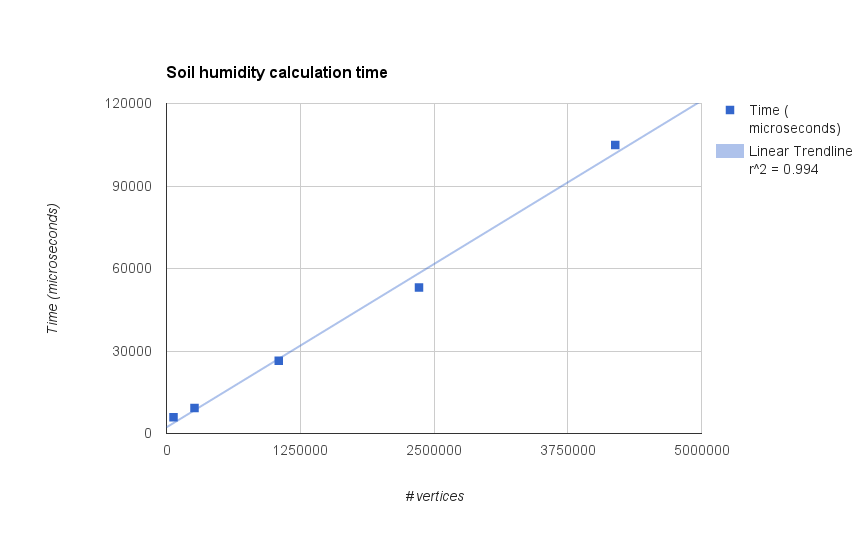
\includegraphics[width=\textwidth]{soil_humidity_calculation_time.png}
	\caption{ Soil humidity calculation time based on vertex count. Analysis performed for terrains with dimensions: 256 by 256, 512 by 512, 1024 by 1024 and 2048 by 2048. }
	\label{fig:soil_humidity_calculation_time}
\end{figure}


\subsubsection{Weighted Monthly Soil Humidity Calculation}

Monthly soil humidity does not take into account the humidity of previous months and therefore fails to model water retention in the soil. By retaining water in the soil, the drought caused by an arid month can be counteracted to some extent by the precipitation of previous months. To model this, a moving weighted average soil humidity is calculated for each month using equation \ref{eq:weighted_avg_monthly_humidity_calculation}.

\begin{equation} \label{eq:weighted_avg_monthly_humidity_calculation}
	S_{wh}(m) =  (\frac{1}{2} \times S_{h}(m)) + (\frac{1}{3} \times S_{h}(m-1)) + (\frac{1}{6} \times S_{h}(m-2))
\end{equation}
where:
\begin{itemize}
\item \textit{$S_{wh}(m)$} is the weighted soil humidity at month \textit{m}, in mm.\\
\item \textit{$S_{h}(m)$} is the soil humidity at month \textit{m}, in mm. \\
\end{itemize}

Similarly to the monthly humidity, the GPU is used to accelerate the calculation process. By doing so, 4 million vertices (2048 by 2048 terrain) can be processed in 285 milliseconds (\ref{fig:weighted_soil_humidity_calculation_time}). There is a linear relationship between vertex count and calculation time (\ref{fig:weighted_soil_humidity_calculation_time}).

\begin{figure}
\center
	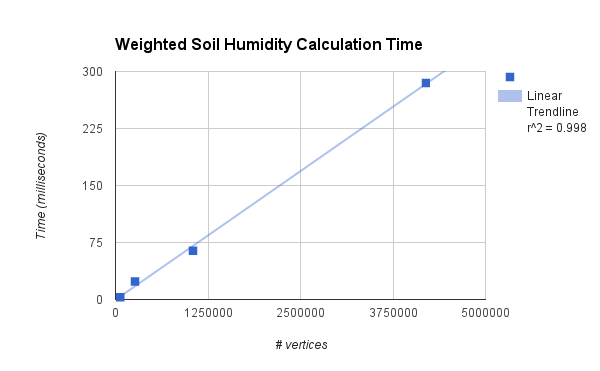
\includegraphics[width=\textwidth]{weighted_soil_humidity_calculation_time.png}
	\caption{ Weighted soil humidity calculation time based on vertex count. Analysis performed for terrains with dimensions: 256 by 256, 512 by 512, 1024 by 1024 and 2048 by 2048. }
	\label{fig:weighted_soil_humidity_calculation_time}
\end{figure}

\subsubsection{Soil Humidity Overlays}

A visual overlay can be displayed to give an overview of both the monthly soil humidity and the weighted average monthly soil humidity on the terrain (see figure \ref{fig:soil_humidity}).

\begin{figure}
\center
	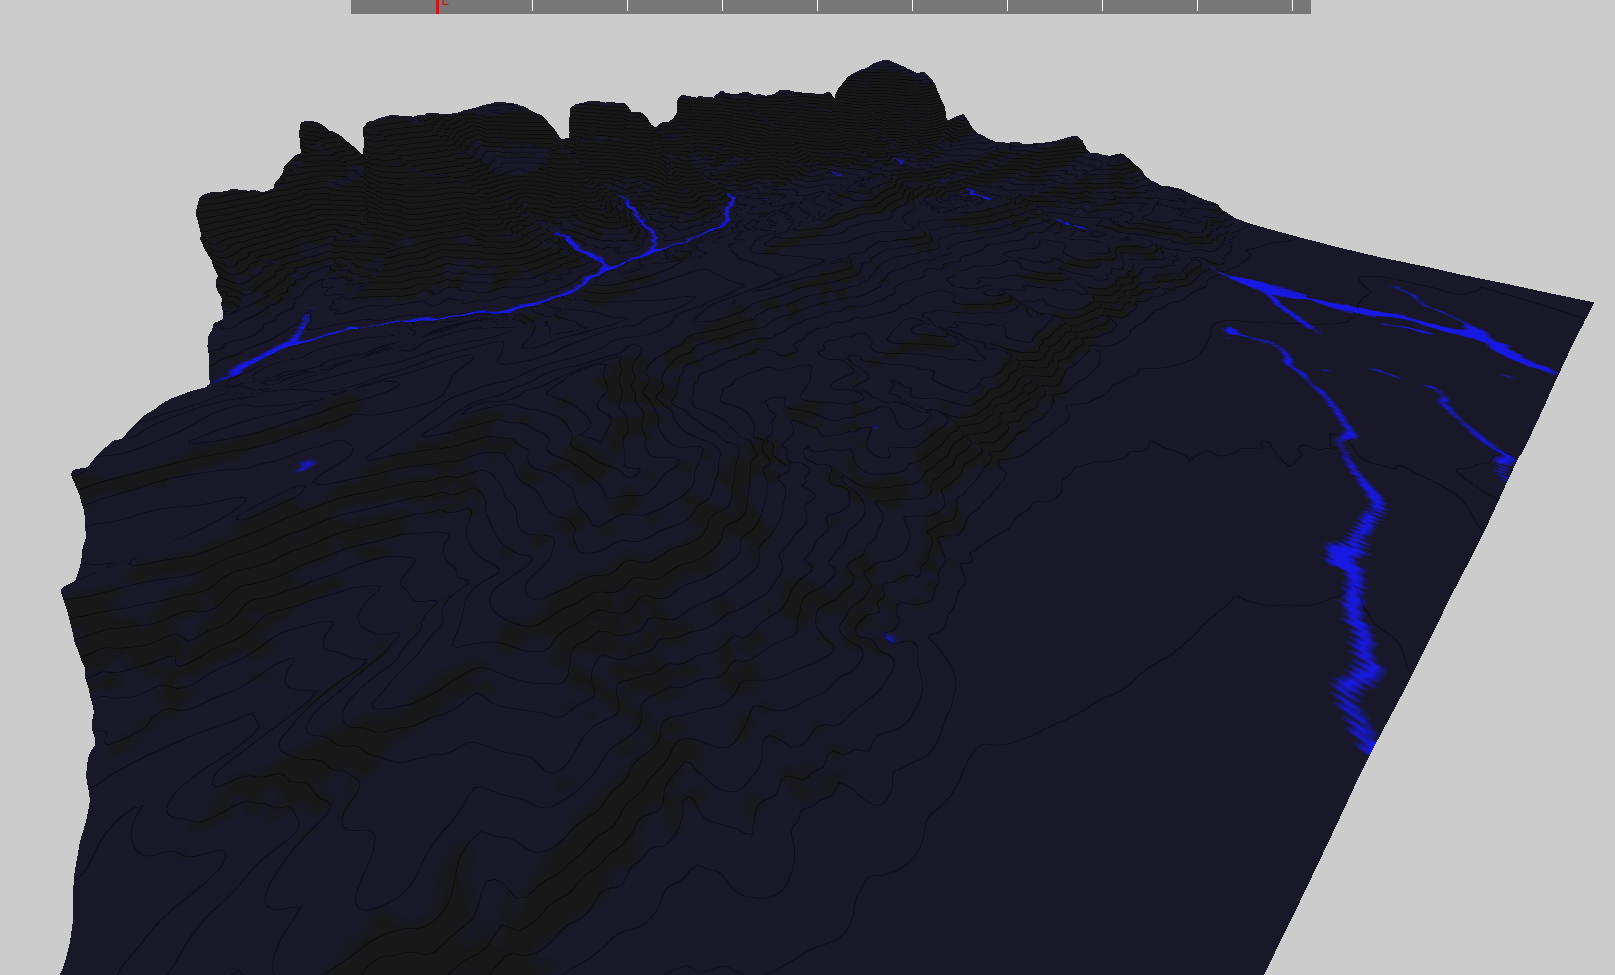
\includegraphics[width=\textwidth]{soil_humidity_overlay.png}
	\caption{ Soil humidity terrain overlay. Colour spectrum ranging from black (zero humidity) to blue (standing water). }
	\label{fig:soil_humidity overlay}
\end{figure}

\subsection{Slope}

Some plants, especially those with a big biomass, can struggle to grow on steep slopes. This is clearly visible in nature, where only smaller plants (shrub, grass, etc.) grow on steeper landscapes. To determine suitable vegetation given the terrain relief, it is therefore important to model slope.\\

This is calculated in real-time using the GPU (34 milliseconds for 4 million vertices) and the relation between vertex count and calculation time is linear (\ref.

\begin{figure}
\center
	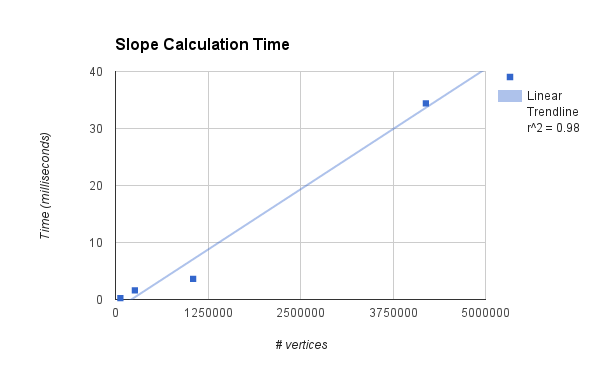
\includegraphics[width=\textwidth]{slope_calculation_time.png}
	\caption{ Slope calculation time based on vertex count. Analysis performed for terrains with dimensions: 256 by 256, 512 by 512, 1024 by 1024 and 2048 by 2048.  }
	\label{fig:slope_calculation_time}
\end{figure}

\subsubsection{Slope Overlay}

To better visualize the slope throughout the terrain, a \textit{slope overlay} can be enabled (see figure \ref{fig:slope overlay}).

\begin{figure}
\center
	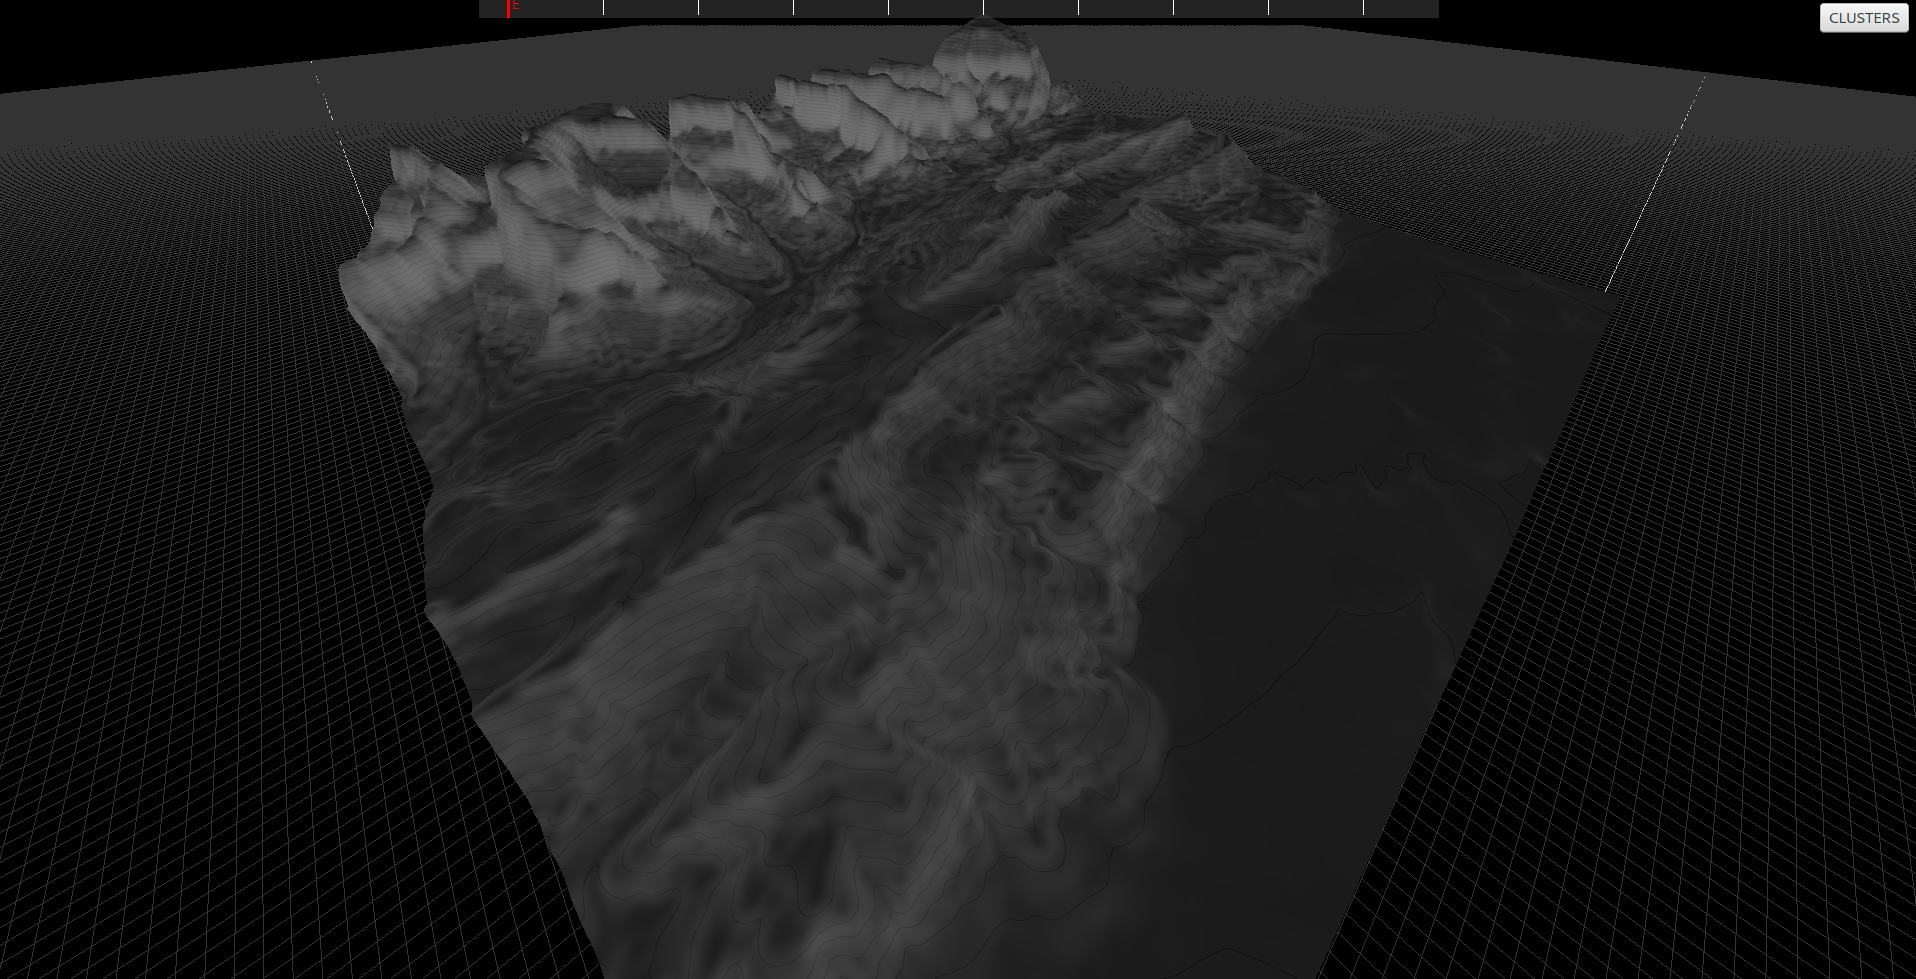
\includegraphics[width=\textwidth]{slope_overlay.png}
	\caption{ Slope visual overlay. Colour spectrum ranging from black (zero degree slope) to white (90 degree slope). }
	\label{fig:slope overlay}
\end{figure}